\documentclass[12pt]{article}
%%---------------------------------------------------------------------
% packages
% geometry
\usepackage{geometry}
% font
\usepackage{fontspec}
\defaultfontfeatures{Mapping=tex-text}  %%如果没有它,会有一些 tex 特殊字符无法正常使用,比如连字符。
\usepackage{xunicode,xltxtra}
\usepackage[BoldFont,SlantFont,CJKnumber,CJKchecksingle]{xeCJK}  % \CJKnumber{12345}: 一万二千三百四十五
\usepackage{CJKfntef}  %%实现对汉字加点、下划线等。
\usepackage{pifont}  % \ding{}
% math
\usepackage{amsmath,amsfonts,amssymb}
% color
\usepackage{color}
\usepackage{xcolor}
\definecolor{EYE}{RGB}{199,237,204}
\definecolor{FLY}{RGB}{128,0,128}
\definecolor{ZHY}{RGB}{139,0,255}
% graphics
\usepackage[americaninductors,europeanresistors]{circuitikz}
\usepackage{tikz}
\usetikzlibrary{positioning,arrows,shadows,shapes,calc,mindmap,trees,backgrounds}  % placements=positioning
\usepackage{graphicx}  % \includegraphics[]{}
\usepackage{subfigure}  %%图形或表格并排排列
% table
\usepackage{colortbl,dcolumn}  %% 彩色表格
\usepackage{multirow}
\usepackage{multicol}
\usepackage{booktabs}
\usepackage{tcolorbox}
% code
\usepackage{fancyvrb}
\usepackage{listings}
\lstset{language=C++}%这条命令可以让LaTeX排版时将C++键字突出显示
\lstset{breaklines}%这条命令可以让LaTeX自动将长的代码行换行排版
\lstset{extendedchars=false}
% title
\usepackage{titlesec}
% head/foot
\usepackage{fancyhdr}
% ref
\usepackage{hyperref}
% pagecolor
\usepackage[pagecolor={EYE}]{pagecolor}
% tightly-packed lists
\usepackage{mdwlist}

\usepackage{../styles/iplouccfg}
\usepackage{../styles/zhfontcfg}
\usepackage{../styles/iplouclistings}

%%---------------------------------------------------------------------
% settings
% geometry
\geometry{left=2cm,right=1cm,top=2cm,bottom=2cm}  %设置 上、左、下、右 页边距
\linespread{1.5} %行间距
% font
\setCJKmainfont{Adobe Kaiti Std}
%\setmainfont[BoldFont=Adobe Garamond Pro Bold]{Apple Garamond}  % 英文字体
%\setmainfont[BoldFont=Adobe Garamond Pro Bold,SmallCapsFont=Apple Garamond,SmallCapsFeatures={Scale=0.7}]{Apple Garamond}  %%苹果字体没有SmallCaps
\setCJKmonofont{Adobe Fangsong Std}
% graphics
\graphicspath{{../figures/}}
\tikzset{
    % Define standard arrow tip
    >=stealth',
    % Define style for boxes
    punkt/.style={
           rectangle,
           rounded corners,
           draw=black, very thick,
           text width=6.5em,
           minimum height=2em,
           text centered},
    % Define arrow style
    pil/.style={
           ->,
           thick,
           shorten <=2pt,
           shorten >=2pt,},
    % Define style for FlyZhyBall
    FlyZhyBall/.style={
      circle,
      minimum size=6mm,
      inner sep=0.5pt,
      ball color=red!50!blue,
      text=white,},
    % Define style for FlyZhyRectangle
    FlyZhyRectangle/.style={
      rectangle,
      rounded corners,
      minimum size=6mm,
      ball color=red!50!blue,
      text=white,},
    % Define style for zhyfly
    zhyfly/.style={
      rectangle,
      rounded corners,
      minimum size=6mm,
      ball color=red!25!blue,
      text=white,},
    % Define style for new rectangle
    nrectangle/.style={
      rectangle,
      draw=#1!50,
      fill=#1!20,
      minimum size=5mm,
      inner sep=0.1pt,}
}
\ctikzset{
  bipoles/length=.8cm
}
% code
\lstnewenvironment{VHDLcode}[1][]{%
  \lstset{
    basicstyle=\footnotesize\ttfamily\color{black},%
    columns=flexible,%
    framexleftmargin=.7mm,frame=shadowbox,%
    rulesepcolor=\color{blue},%
%    frame=single,%
    backgroundcolor=\color{yellow!20},%
    xleftmargin=1.2\fboxsep,%
    xrightmargin=.7\fboxsep,%
    numbers=left,numberstyle=\tiny\color{blue},%
    numberblanklines=false,numbersep=7pt,%
    language=VHDL%
    }\lstset{#1}}{}
\lstnewenvironment{VHDLmiddle}[1][]{%
  \lstset{
    basicstyle=\scriptsize\ttfamily\color{black},%
    columns=flexible,%
    framexleftmargin=.7mm,frame=shadowbox,%
    rulesepcolor=\color{blue},%
%    frame=single,%
    backgroundcolor=\color{yellow!20},%
    xleftmargin=1.2\fboxsep,%
    xrightmargin=.7\fboxsep,%
    numbers=left,numberstyle=\tiny\color{blue},%
    numberblanklines=false,numbersep=7pt,%
    language=VHDL%
    }\lstset{#1}}{}
\lstnewenvironment{VHDLsmall}[1][]{%
  \lstset{
    basicstyle=\tiny\ttfamily\color{black},%
    columns=flexible,%
    framexleftmargin=.7mm,frame=shadowbox,%
    rulesepcolor=\color{blue},%
%    frame=single,%
    backgroundcolor=\color{yellow!20},%
    xleftmargin=1.2\fboxsep,%
    xrightmargin=.7\fboxsep,%
    numbers=left,numberstyle=\tiny\color{blue},%
    numberblanklines=false,numbersep=7pt,%
    language=VHDL%
    }\lstset{#1}}{}
% pdf
\hypersetup{pdfpagemode=FullScreen,%
            pdfauthor={Haiyong Zheng},%
            pdftitle={Title},%
            CJKbookmarks=true,%
            bookmarksnumbered=true,%
            bookmarksopen=false,%
            plainpages=false,%
            colorlinks=true,%
            citecolor=green,%
            filecolor=magenta,%
            linkcolor=cyan,%red(default)
            urlcolor=cyan}
% section
%http://tex.stackexchange.com/questions/34288/how-to-place-a-shaded-box-around-a-section-label-and-name
\newcommand\titlebar{%
\tikz[baseline,trim left=3.1cm,trim right=3cm] {
    \fill [cyan!25] (2.5cm,-1ex) rectangle (\textwidth+3.1cm,2.5ex);
    \node [
        fill=cyan!60!white,
        anchor= base east,
        rounded rectangle,
        minimum height=3.5ex] at (3cm,0) {
        \textbf{\thesection.}
    };
}%
}
\titleformat{\section}{\Large\bf\color{blue}}{\titlebar}{0.1cm}{}
% head/foot
\setlength{\headheight}{15pt}
\pagestyle{fancy}
\fancyhf{}
%\lhead{\color{black!50!green}2014年秋季学期}
\chead{\color{black!50!green}Zooplankton Attributes}
%\rhead{\color{black!50!green}通信电子电路}
\lfoot{\color{blue!50!green}王如晨\ 朱亚菲}
\cfoot{\color{blue!50!green}\href{http://vision.ouc.edu.cn/~zhenghaiyong}{CVBIOUC}}
\rfoot{\color{blue!50!green}$\cdot$\ \thepage\ $\cdot$}
\renewcommand{\headrulewidth}{0.4pt}
\renewcommand{\footrulewidth}{0.4pt}


%%---------------------------------------------------------------------
\begin{document}
%%---------------------------------------------------------------------
%%---------------------------------------------------------------------
% \titlepage
\title{\vspace{-2em}浮游动物特征总结\vspace{-0.7em}}
\author{王如晨\ 朱亚菲}
\date{\vspace{-0.7em}2015年8月\vspace{-0.7em}}
%%---------------------------------------------------------------------
\maketitle\thispagestyle{fancy}
%%---------------------------------------------------------------------
\maketitle
\tableofcontents 

%形态学是生物分类学的主要依据。
\section{13类浮游动物的特征}
\begin{description}
    \item[Appendicularia(尾海鞘纲)] 属于脊索动物门,体型像蝌蚪,身体分为躯干和尾两部分。躯干为椭圆形;尾部扁平,比躯干要长。\footnote{\url{https://zh.wikipedia.org/wiki/\%e5\%b0\%be\%e6\%b5\%b7\%e9\%9e\%98\%e7\%ba\%b2}} 大小:小于5mm。
    
    观察采集的图像发现:
    \begin{itemize}
        \item 形状像蝌蚪,分为躯干和尾部。
        \item 躯干较大且灰度较深,并不是呈现规则的椭圆(还有部分突出了的东西还不知道是什么)。
        \item 尾部大致呈现两种形状:一种细长弯曲;另一种较粗(粗细甚至于头部差不多),呈现柳叶状。尾部的灰度相比于躯干较浅,轮廓不太清晰。
    \end{itemize}
    \item[Bubble(气泡)] 非生物。
    
    观察采集的图像发现:
        \begin{itemize}
        \item 圆形。
        \item 气泡四周灰度深,中间灰度很浅,呈亮白色。
        \end{itemize}
    \item[Chaetognatha(毛颚动物门)] 全体分为头、躯干和尾3部分。头部略膨大,躯干与头连接处稍微缢缩为颈部,尾部末端尖细。头部两侧各着生一列4~13根镰刀状、几丁质的颚毛。\footnote{\url{https://zh.wikipedia.org/wiki/\%e6\%af\%9b\%e9\%a2\%9a\%e5\%8a\%a8\%e7\%89\%a9\%e9\%97\%a8}}大小:最大成年成年个体长105mm,该类成年个体的长度一般都大于5mm。
    
    观察采集的图像发现:
        \begin{itemize}
        \item 身体修长,可以明显看出身体分为头、躯干和尾三部分。
        \item 头部小且圆滑,在头与躯干连接的地方略窄。
        \item 躯干较粗,轮廓清晰。
        \item 尾部慢慢变窄,末尾尖。
        \end{itemize}
    \item[{\color{blue}Cladocera Penilia(Penilia avirostris,鸟喙尖头溞)}] 属于节肢动物门,鳃足纲,枝角目,俗称水跳蚤。大小:大约为1mm左右。
    
    观察采集的图像发现:长圆形,大部分图像可以看到一对较长的触角,并且中轴灰度较深。
    \item[{\color{blue}Copepoda(桡脚类)}] 属于节肢动物门,颚足纲。体形像泪珠,有大的触角。分为前体部和后体部,前体部较为宽大,后体部较为短小。\footnote{\url{https://zh.wikipedia.org/wiki/\%e6\%a9\%88\%e8\%85\%b3\%e9\%a1\%9e}}前体部前体部由头和胸部组成,头部有两对触角,胸部有鄂足、五对胸足。后体部无附肢,由3—5节组成。最末的腹节称尾节,末端具1对尾叉,尾叉的末端有5根不等长的刚毛,常呈羽状。\footnote{\url{http://baike.baidu.com/view/665478.htm}}
    
    观察采集的图像发现:身体类似椭圆形,身体前部的触角不是特别清晰,身体后部的触角较短,并成簇存在。
    \item[{\color{blue}Decapoda(十足目)}] 属于节肢动物门,软甲纲。分为两类:Lucifer hanseni和Crab larvae。体躯延长呈虾形(腹部发达)或缩短扁圆呈蟹形(腹部化)。\footnote{\url{http://baike.baidu.com/link?url=LWmrgD_DVUcw0upg_zi0LTIJWj6quxa_juRrS3zUt91A-FjPM6VQwYfZ5fFZckzIyEGCaXyS_pikXUGg2JsYMXUX-uFEkmkLqC5lfkxvXvApK3WRBcWQkfbDhMlfTdgrWvh-728gSoUylWZG2UstFK}}
    
    观察采集的图像发现:形状大致分为虾形和蟹形。
    \item[Doliolida(海樽目)] 属于脊索动物门,樽海鞘纲\footnote{\url{https://zh.wikipedia.org/wiki/\%e6\%a8\%bd\%e6\%b5\%b7\%e9\%9e\%98\%e7\%ba\%b2}}。体型一般呈桶状,体壁最外是被囊层,其内层是外套膜。被囊层下有8~9条肌带环绕着体躯。
    
    观察采集的图像发现:
        \begin{itemize}
        \item 由于该类浮游动物比较透明,因此在图像中灰度较浅,并且其桶状轮廓也不完整了,但最明显的是能看到大概7、8条环状的肌肉带,有的图像中还能看到内部器官。
        \end{itemize}
    \item[{\color{blue}Egg}] 鱼卵以及其他浮游动物的卵。
    
    观察采集的图像发现:
        \begin{itemize}
        \item 形状大致都呈圆形。
        \item 有的卵整体灰度都很深;有的卵中间有一块灰度较深的区域,四周灰度较浅(结构像细胞)。
        \end{itemize}
    \item[Fiber(纤维)] 非生物。
        \begin{itemize}
        \item 弯曲的线状,有的纤维有分叉和交叉。
        \item 该类图像中噪声较多,纤维的边缘也不是很规则。
        \end{itemize}
    \item[Gelatinous(明胶)] 胶质的浮游动物,包括Aglaura(属于刺胞动物门,这一个没有搜的中文名字,但也属于水母类)、Medusa(水母,属于刺胞动物门,水螅纲)、Siphonophora(管水母,属于刺胞动物门,水螅纲,管水母目)、Radiolaria(放射虫,属于原声动物门,辐足纲)和Salps(樽海鞘,属于脊索动物门Chordata,樽海鞘纲Thaliacea,纽鳃樽目Salpida)。该类是多种呈胶质浮游动物的集合。大部分水母都有三个主要部位:圆伞状或是钟状(寺院里面敲得那种钟)的身体﹐触器和口腕。
    
    观察采集的图像发现:
        \begin{itemize}
        \item 由于该类呈胶状,因此该类物体灰度整体较浅,边缘也不是十分清晰。大部分是水母,有小部分的樽海鞘(与海樽目形态很相似),小部分的放射虫。
        \item 其中水母也包括很多类,形态大致呈现以下几种:
            \begin{itemize}
            \item 一些水母身体呈现类似钟状(这里呈现钟状有长有短,有粗有细,还有的会发生一点弯曲),灰度较浅,内部有一块颜色较深的椭圆形区域。
            \item 一些水母也呈钟状,但内部没有颜色较深的椭圆形区域,整个身体灰度均匀。
            \item 还有的个头稍微偏小,形状有的类似圆形、像半个胶囊(应该是由于拍摄原因,有的拍到顶部,有的拍到侧面),体内有颜色较深的一个大点和几个小点。(可能是灯塔水母)
            \item 还有四张看不出形状的,不知道是什么。
            \end{itemize}
        \item 放射虫:形状近似圆形(但由于整体灰度较浅,形状保存是完整),中间有一块灰度较深的区域,四周灰度较浅,可以看到淡淡的细纹从中心连接到边界。
        \end{itemize}
    \item[{\color{blue}Multiple(多个生物)}] 由于浮游动物的重叠,导致分割过程中多个浮游动物被分割到一张图像上。
    \item[{\color{blue}Nonbio}] 非生物的集合。
    \item[Pteropoda(翼足目)] 属于软体动物门,腹足纲。
    
    观察采集的图像发现:
    \begin{itemize}
    \item 该类浮游动物灰度较深,形状总体都呈现一头宽一头窄。
    \item 形状总体呈现三类:有的呈现象牙状,有点弯曲;有的较粗短,像一顶尖的小帽子;有的呈现细长的三角形状。
    \end{itemize}
\end{description}

参考网站:\url{http://www.imas.utas.edu.au/zooplankton/home}。

\section{PkID中用到的特征}
PkID中用到的特征一共有67个:Area, Mean, StdDev, Mode, Min, Max, X, Y, XM, YM, Perim., BX, BY, Width, Height, Major, Minor, Angle, Circ., Feret, IntDen, Median, Skew, Kurt, \%Area, XStart, YStart, Area\_exc, Fractal, Skelarea, Slope, Histcum1, Histcum2, Histcum3, XMg5, YMg5, Compentropy, Compmean, Compslope, CompM1, CompM2, CompM3, Symetrieh, Symetriev,Tag, ESD, Elongation, Range, MeanPos, CentroidsD, CV, SR, PerimAreaexc, FeretAreaexc, PerimFeret, PerimMaj, Circexc, CDexc, {\color{blue}Nb1, Nb2, Nb3,  Symetriehc, Symetrievc, Convperim, Convarea, Fcons, ThickR(这几个特征没有找到具体的含义)}

从训练集的PID文件文件中看到,Compentropy, Compmean, Compslope, CompM1, CompM2, CompM3这6个特征在所有图像上的值都为0,Tag这个特征在所有图像上的值都为1,在训练分类器时是不起作用的,同时这7个特征的具体含义也没有找到。

\subsection{位置特征}
\begin{description}
\item[BX] 能够包围物体,且平行于图像两条边的最小外界矩形的左上角顶点的X坐标 
\item[BY] 能够包围物体,且平行于图像两条边的最小外界矩形的左上角顶点的Y坐标 
\item[Height] 能够包围物体,且平行于图像两条边的最小外界矩形的高
\item[Width] 能够包围物体,且平行于图像两条边的最小外界矩形的宽
\item[XStart] 图像最左上角像素点的X坐标
\item[YStart] 图像最左上角像素点的Y坐标
\item[XM] 物体灰度重心的X坐标
\item[YM] 物体灰度重心的Y坐标
\item[XMg5] gamma值为51时的物体灰度重心的X坐标(gamma值表示图像输出值与输入值关系的斜率)
\item[YMg5] gamma值为51时的物体灰度重心的Y坐标
\item[X] 物体重心点的X坐标
\item[Y] 物体重心点的Y坐标
\item[Angle] 浮游动物主轴与图片x轴形成的夹角,在图片切割后旋转图片测量相关参数使用
\end{description}

这类特征反映的是浮游动物在图像中的位置信息,浮游动物特征与位置信息无关,因此它们不适合作为特征直接用于分类(会降低分类的准确率),而是用来计算其他特征(尺寸特征、灰度特征和形状特征)。

\subsection{尺寸特征}

\begin{description}
\item[Area] 物体的表面积,方形像素的个数%包含物体的最小矩形面积 
\item[Perim] 周长,物体最外层边缘的长度
\item[Major] 物体的最佳拟合椭圆的长轴%物体内切椭圆的长轴
\item[Minor] 物体的最佳拟合椭圆的短轴%物体内切椭圆的短轴
\item[Feret] Maximum feret diameter(最大费雷特径), 沿物体边缘任意两个点的最长距离
\item[Area\_exc] 去掉物体空洞后的表面积,空洞是指灰度值与背景相同的部分
\item[\%area] 物体表面积中空洞所占的百分比,即背景所占的比例
\end{description}

这类特征表示了图像中目标的大小尺寸。它的根据是同类浮游动物的表面积、周长等尺寸特征应该是大致相同的。但是这些特征还存在着问题:1、同类浮游动物在不同时期(如幼年和成年)的个体大小尺寸是不同的。2、拍摄照片的方位不同(比如正面和侧面)得到的尺寸特征也是不同的。

\subsection{灰度值特征}

\begin{description}
    \item[Min] 物体内部所有像素点的最小灰度值 (0 = black)
    \item[Max] 物体内部所有像素点的最大灰度值 (255 = white)
    \item[IntDen (Integrated density)] 总密度,物体内像素点的灰度值的总和($IntDen = Area * Mean$)
    \item[Slope] 归一化的灰度累计直方图的斜率
    \item[Histcum1] 灰度累计直方图的值为25\%时所对应的灰度值
    \item[Histcum2] 灰度累计直方图的值为50\%时所对应的灰度值
    \item[Histcum3] 灰度累计直方图的值为75\%时所对应的灰度值
    \item[CentroidsD] $\sqrt{(XM-X)^{2}+(YM-Y)^{2}}$ 目标物体重心和灰度重心之间的距离。
\end{description}

%这类特征描述的是浮游动物的灰度特征,其中Min、Max、StdDev、Range反映了图像中目标的灰度范围,Skew、Kurt、Slope、Histcum1、Histcum2、Histcum3、Mean、IntDen、Mode、Mean\_exc、Median反映了目标整体的灰度变化和集中趋势,CentroidsD、CV、SR还不清楚它们的物理意义。

根据是同类浮游动物的灰度特征(灰度的范围和整体灰度变换趋势)应该是相似的,但观察图像发现并不是所有同类浮游动物的灰度都是相似的,例如Gelatinous类中有的个体灰度跨度较小,整体灰度都较浅,而有的个体灰度跨度较大;同时由于拍摄时光线的原因,会造成同类浮游动物中个体灰度的深浅不一。

\subsection{形状特征}

\begin{description}
    \item[Fractal] 物体边界的分形维数 (Berube and Jebrak, 1999),表明物体边界的不规则程度
    \item[Skelarea] 骨架像素的表面积(在二值图像中,不断地从物体边缘处减去像素点直到仅剩一个像素的宽度,最后所得图形的像素点数)
    \item[Symetrieh] 水平对称
    \item[Symetriev] 垂直对称
    \item[Circ] $Circularity = (4 * Pi * Area) / Perim^2$ 圆形度,表征物体接近圆的程度,值等于1时,说明物体为正圆形,值越接近0,物体体形越长。
    \item[ESD] $2 \times \sqrt{\cfrac{Area}{\pi}}$ 相应球形直径(也称为等效球直径),是指一不规则外形物体,其体积相同球体的直径。
    \item[Elongation] $\cfrac{Major}{Minor}$ 延伸率,最佳拟合椭圆的长轴和短轴之比。
    \item[Circexc] $\cfrac{4 \times \pi Area\_exc}{Perim^{2}}$ 去掉目标内部空洞的圆形度。
\end{description}

这类特征描述的是浮游动物的灰度特征,根据的是不同种类浮游动物的形状不同。存在的问题是有不同种类的浮游动物形状相似,例如Appendicularia和Chaetognatha,Bubble和Egg;也有同种浮游动物形状不同,例如Decapoda、Gelatinous。

\subsection{生物统计特征}

\begin{description}
    \item[Mean] 物体内的平均灰度值;物体中所有像素点的灰度值的总和除以总的像素个数    
    \item[Range] $Max-Min$ 极差,灰度的范围。    
    \item[CV] $100 \times \cfrac{StdDev}{Mean}$ 变异系数(也称离散系数或相对偏差),是灰度标准偏差与平均值之比,用百分数表示。
    \item[SR] $100 \times \cfrac{StdDev}{Max-Min}$ 灰度标准差比上极差。
    \item[Skew] 灰度直方图的偏度,衡量灰度分布的不对称性。偏度为负就意味着在概率密度函数左侧的尾部比右侧的长,绝大多数的值位于平均值的右侧。偏度为正就意味着在概率密度函数右侧的尾部比左侧的长,绝大多数的值位于平均值的左侧。偏度为零就表示数值相对均匀地分布在平均值的两侧,但不一定意味着其为对称分布。
    \item[Kurt] 峰度,描述灰度直方图的陡缓程度。 
    \item[Mean\_exc] 物体内部去掉空洞后的平均灰度值 ($Mean\_exc = IntDen / Area\_exc$)
    \item[Median] 物体内像素的灰度值的中值
    \item[StdDev] 物体内像素的灰度值的标准差
    \item[Mode] Modal grey value within the object(可能表示灰度的众数)
\end{description}

\subsection{还没有查找到的特征}
\begin{description}
    \item[MeanPos] $\cfrac{Mean-Max}{Max-Min}$
    \item[PerimAreaexc] $\cfrac{Perim}{\sqrt{Area\_exc}}$ 
    \item[FeretAreaexc] $\cfrac{Feret}{\sqrt{Area\_exc}}$
    \item[PerimFeret] $\cfrac{Perim}{Feret}$
    \item[PerimMaj] $\cfrac{Perim}{Major}$
    \item[CDexc] $\cfrac{\sqrt{(XM-X)^{2}+(YM-Y)^{2}}}{{\sqrt{Area\_exc}}}$ 
\end{description}

\subsection{其他特征}
这些特征并没有在PkID中使用,而是在作者的一个幻灯片中提到的新特征。
\begin{description}
\item[Texture Contrast] 
\item[Cumulation Histogram]
\item[Convex Area]
\item[Symmetry]
\item[Thickness Ratio]
\end{description}


\subsection{实验}
\subsubsection{PkID+RandomForest}
采用以上67个特征,并用随机森林分类器进行训练和分类得到的混淆矩阵如图~\ref{fig: PkID-RF-2-folds-5-repetitions}。

\begin{figure}[!ht]
\centering
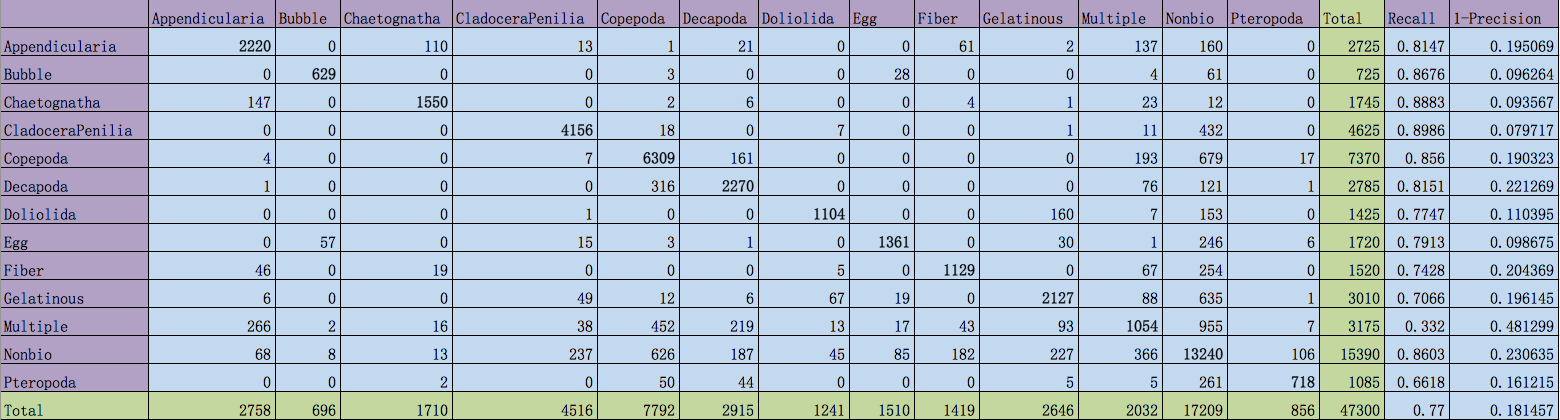
\includegraphics[width=1.0\linewidth]{PkID-RF-2-folds-5-repetitions}
\caption{PkID-RF交叉验证,folds取2,repetitions取5}
\label{fig: PkID-RF-2-folds-5-repetitions}
\end{figure}

\subsubsection{PkID+SVM}
PkID系统中SVM Linear的参数如图~\ref{fig:SVM-Linear-Parameters}。
\begin{figure}[!ht]
\centering
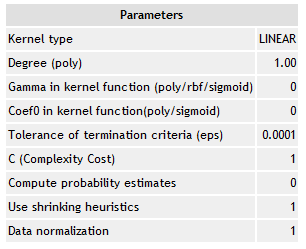
\includegraphics[width=0.4\linewidth]{SVM-Linear-Parameters}
\caption{PkID系统中SVM Linear的参数}
\label{fig:SVM-Linear-Parameters}
\end{figure}

采用以上67个特征,并用SVM分类器进行训练和分类得到的混淆矩阵如图~\ref{fig: PkID-SVM-2-folds-5-repetitions}。
\begin{figure}[!ht]
\centering
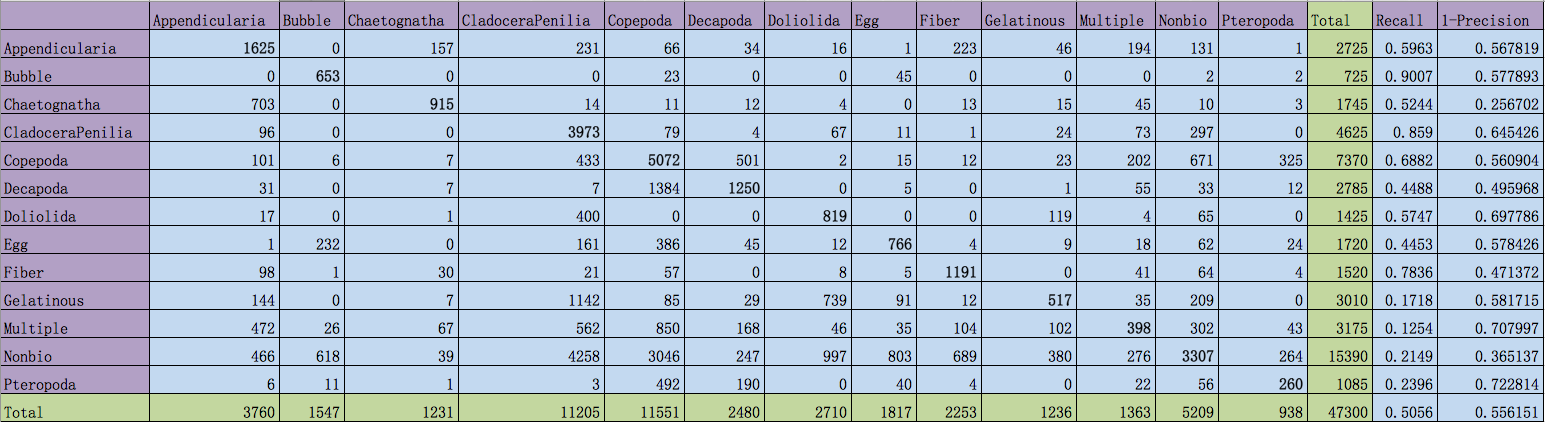
\includegraphics[width=1.0\linewidth]{PkID-SVM-2-folds-5-repetitions}
\caption{PkID-SVM交叉验证,folds取2,repetitions取5}
\label{fig: PkID-SVM-2-folds-5-repetitions}
\end{figure}






\section{计算机视觉特征提取}

\subsection{几何参数}

\subsubsection{边界的周长}
轮廓边界的周长。对轮廓边缘上的像素点的统计。

\subsubsection{边界的曲率}

\subsubsection{面积}
描述区域大小的特征。对区域内总像素点的统计。

\subsubsection{宽度和高度}
最小外接矩形的宽度和高度

\subsubsection{矩形度}
反映被检测目标的最小外接矩形的充满程度,当目标的形状越接近矩形时,矩形度的值越接近1。
    \begin{displaymath}
    R=\frac{A}{WH}
    \end{displaymath}
    A为目标的面积,W、H分别为最小外接矩形的宽度和高度。

\subsubsection{体态比}
为目标最小外接矩形的长与宽的比值。
    \begin{displaymath}
    C=\frac{W}{H}
    \end{displaymath}
    
\subsubsection{圆形性}
用目标区域的所有边界点定义的特征向量。
    \begin{displaymath}
    C_{I}=\frac{\mu_{R}}{\sigma_{R}}
    \end{displaymath}
    $\mu_{R}$为区域重心到边界点的平均距离,$\sigma_{R}$为从区域重心到边界点的距离的平均方差。

\subsubsection{偏心率}
在一定程度上反映了区域的紧凑程度。定义为目标区域长短主轴的平方根的比值。
    \begin{displaymath}
    E=\frac{p}{q}
    \end{displaymath}
    设目标区域在XY平面上,区域像素点绕X轴的转动惯量为A,绕Y轴的转动惯量为B,惯性积为C。目标区域的长度分别是p和q。
    \begin{displaymath}
    p=\sqrt{\frac{2}{(A+B)+\sqrt{(A-B)^{2}+4C^{2}}}}
    \end{displaymath}
    \begin{displaymath}
    q=\sqrt{\frac{2}{(A+B)-\sqrt{(A-B)^{2}+4C^{2}}}}
    \end{displaymath}
    
\subsubsection{凸率}
为目标区域面积与目标区域凸包面积之比,该特征包含着描述边界不规则特性的信息。
    \begin{displaymath}
    C_{R}=\frac{A}{\sum_{x=1}^{M}\sum_{y=1}^{N}k(x,y)}
    \end{displaymath}
    分母为凸包区域的面积。
    
\subsubsection{密集度}
描述目标密集度的量化特征,提供了目标形状的重要信息。在周长确定后,密集度越高,所围成的面积越大。
    \begin{displaymath}
    C_{2}=\frac{L^{2}}{4\pi A}
    \end{displaymath}
    L为周长。
    
\subsubsection{球状性}
内切圆的直径与外接圆的直径之比。
    \begin{displaymath}
    S=\frac{r_{i}}{r_{c}}
    \end{displaymath}
    
\subsubsection{伸长度}
周长与目标区域最小外接矩形面积之比。
    \begin{displaymath}
    P=\frac{L}{WH}
    \end{displaymath}

\subsubsection{叶状性}
叶状反映了边界的幅度特征,为区域重心到边界的最短距离与目标区域的最大宽度之比。
    \begin{displaymath}
    B=\frac{R_{1}}{W_{max}}
    \end{displaymath}
    
\subsection{几种典型的特征描述方法}

\subsubsection{边界描述子}
\begin{itemize}
\item 链码
\item 多边形近似
\item 骨架
\item 形状数
\item 统计矩:边界线段的形状可以通过简单的统计矩进行定量的描述,如均值、方差和高阶矩。
\item 傅里叶描述子
\item 曲率尺度空间
\item 形状上下文(KNN)
\end{itemize}

\subsubsection{区域描述子}
\begin{itemize}
\item 拓扑描述:欧拉数
\item 不变矩
\item 角半径变换(Angular RadialTransformation, ART):通过使用一组半径变换系数,描述单个连通区域或者不连通区域,对旋转和噪声具有鲁棒性。
\item 纹理
    \begin{itemize}
    \item 统计方法:灰度共生矩阵
    \item 模型法:马尔科夫随机场
    \item 频谱方法:Gabor滤波、小波变换
    \end{itemize}
\end{itemize}

\begin{comment}
\subsection{经典特征描述方法}

\subsubsection{SIFT特征}

\subsubsection{HOG特征}

\subsubsection{LBP特征}

\subsubsection{Shape Context}

\subsubsection{Fisher Vector}
\end{comment}

\subsection{特征融合}
特征融合分为三个层次:数据级融合、特征级融合和决策级融合。
数据级融合是结合未加工的信息来得到更加丰富的信息。
特征级融合是选择并结合特征来去除多余和无关的特征。
决策级融合是用多个相同或不同的分类器,相同或不同的分类器。

图像融合方法:

像素级:PCA(主成分分析)、HIS变换、Brovery变换、线性加权法、SFIM、IHS变换、高通滤波法、小波变换融合算法。

特征级:聚类分析法、贝叶斯估计法、信息熵法、神经网络法、带权平均法、Dempster-shafer推理法、表决法及神经网络法。

决策级:神经网络法、贝叶斯融合、模糊聚类法、模糊集理论、可靠性理论以及逻辑模板法。

\subsubsection{贝叶斯融合(Bayes Fusion)}
当在进行图像分类过程中,可能需要用到不止一种特征。贝叶斯融合可以通过结合不同分类器的结果实现特征融合。

\textbf{贝叶斯融合规则:}

如果要将一幅图像分类到$n$个可能的种类中($\omega_{1},\dots,\omega_{n}$),$x_{i}$表示第$i$个分类器产生的待识的属性,它属于$n$个模式类之一。记$P(\omega_{k})$为先验概率,$P(x_{i}|\omega_{k})$为每类的概率密度函数,$P(x_{1},\dots,x_{R}|\omega_{k})$联合概率分布函数,$R$为用来分类的分类器数目。

根据贝叶斯最小错误率理论,如果
\begin{equation}
P(\omega_{j}|x_{1},\dots,x_{R})=\max_{k}P(\omega_{k}|x_{1},\dots,x_{R})
\end{equation}
则$Z\in\omega_{j}$。

且有:
\begin{equation}
P(\omega_{j}|x_{1},\dots,x_{R})=\frac{P(x_{1},\dots,x_{R}|\omega_{k})P(\omega_{k})}{P(x_{1},\dots,x_{R})}
\end{equation}
其中
\begin{equation}
P(x_{1},\dots,x_{R})=\sum^{n}_{j=1}P(x_{1},\dots,x_{R}|\omega_{k})P(\omega_{j})
\end{equation}
假定分类器度量之间是相互独立的,有:
\begin{equation}
P(x_{1},\dots,x_{R}|\omega_{k})=\prod^{R}_{i=1}P(x_{i}|\omega_{k})
\end{equation}
将式(3)(4)带入式(2)有:
\begin{equation}
P(\omega_{j}|x_{1},\dots,x_{R})=\frac{P(\omega_{k})\prod^{R}_{i=1}P(x_{i}|\omega_{k})}{\sum^{n}_{j=1}P(\omega_{j})\prod^{R}_{i=1}P(x_{i}|\omega_{k})}
\end{equation}
将式(5)带入式(1),得到:
\begin{enumerate}
\item 融合规则1:乘法规则
    \begin{equation}
    P(\omega_{j})\prod^{R}_{i=1}P(x_{i}|\omega_{j})=\max^{n}_{k=1}P(\omega_{k})\prod^{R}_{i=1}P(x_{i}|\omega_{k})
    \end{equation}
    转化为后验概率,得到:
    \begin{equation}
    P^{-(R-1)}(\omega_{j})\prod^{R}_{i=1}P(\omega_{j}|x_{i})=\max^{n}_{k=1}P^{-(R-1)}(\omega_{k})\prod^{R}_{i=1}P(\omega_{k}|x_{i})
    \end{equation}
    这样就可以将该图片归类为$\omega_{j}$。
\item 融合规则2:加法规则

    在乘法规则中,如果假定由分类器输出的后验概率与相应的先验概率之间只有微小的偏差:
    \begin{equation}
    P(\omega_{k}|x_{i})=P(\omega_{k})(1+\delta_{ki}), \delta_{ki}\ll1
    \end{equation}
    由此得到:
    \begin{equation}
    P^{-(R-1)}(\omega_{k})\prod^{R}_{i=1}P(\omega_{k}|x_{i})=P(\omega_{k})\prod^{R}_{i=1}(1+\delta_{ki})
    \end{equation}
    如果将上式右边的乘积展开忽略二次以上的项,即:
    \begin{equation}
    P(\omega_{k})\prod^{R}_{i=1}(1+\delta_{ki})=P(\omega_{k})+P(\omega_{k})\sum^{R}_{i=1}\delta_{ki}
    \end{equation}
    再将式(8)(10)带入(7)可以得到加法规则如下:
    \begin{equation}
    (1-R)P(\omega_{j})+\sum^{n}_{i=1}P(\omega_{j}|x_{i})=\max^{n}_{k=1}[(1-R)P(\omega_{k})+\sum^{R}_{i=1}P(\omega_{k}|x_{i})]
    \end{equation}
    通常我们假定各类的先验概率是相等的,则上式等价于:
    \begin{equation}
    \sum^{R}_{i=1}P(\omega_{j}|x_{i})=\max^{n}_{k=1}\sum^{R}_{i=1}P(\omega_{k}|x_{i})
    \end{equation}
    由于加法规则对估计误差不敏感,因而具有比其他规则更好的性能。
\end{enumerate}


\begin{comment}
\begin{itemize}
\item 基于灰度共生矩阵的方法
\item 灰度-梯度共生矩阵分析法
\item 灰度行程长度统计法
\item 小波分析法
\item 基于Gabor小波变换的纹理分析法
\end{itemize}
\end{comment}




\bibliographystyle{plain}

\bibliography{Features} %参考文献

\end{document}
